\chapter{Perancangan}
\label{chap:perancangan}

Bab ini membahas perancangan untuk seluruh fitur yang diimplementasi pada  perangkat lunak SharIF Judge.

\section{Rancangan Antarmuka}
\label{sec:4:antarmuka}

\begin{figure}[H]
	\centering  
	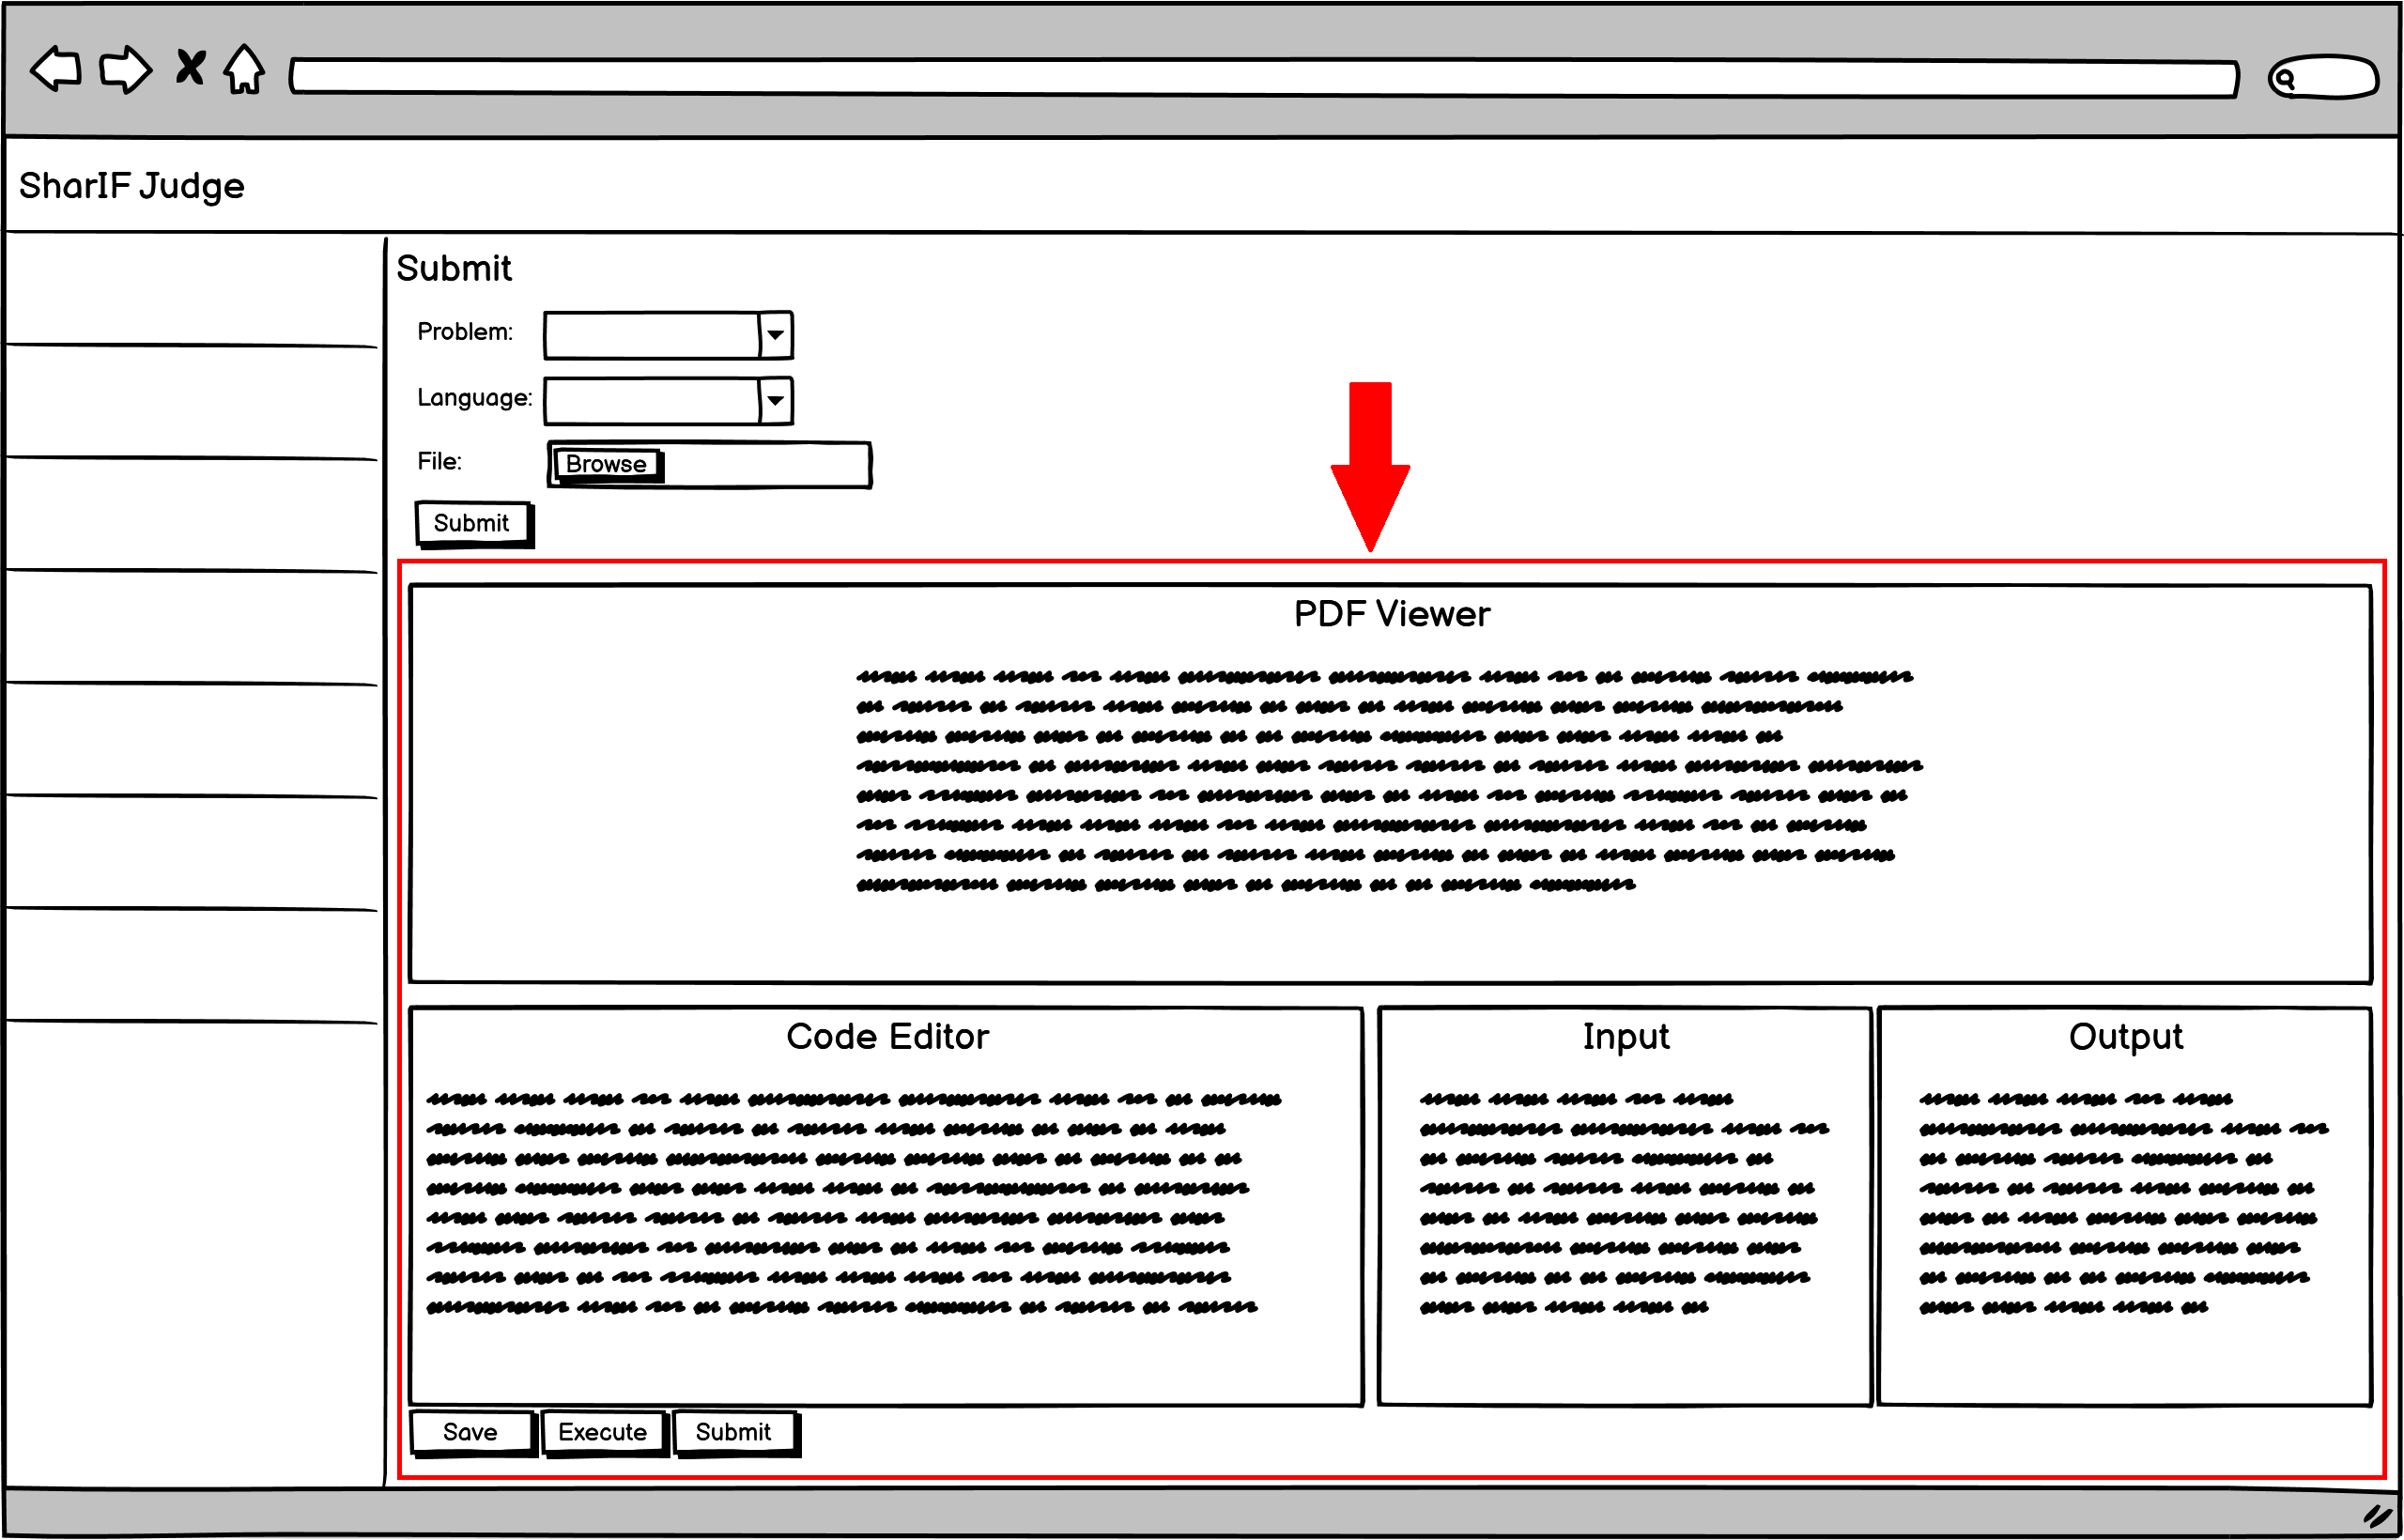
\includegraphics[scale=0.2]{submit_mockup}  
	\caption{Rancangan antarmuka halaman Submit} 
	\label{fig:4:antarmuka} 
\end{figure} 

Seluruh fitur akan diimplementasikan pada halaman Submit. Gambar \ref{fig:4:antarmuka} menunjukkan rancangan antarmuka halaman Submit, dengan tambahan yang diimplementasikan ditandai dengan kotak merah. Pada halaman Submit sudah terdapat \textit{dropdown} untuk memilih \textit{problem} yang akan dikerjakan, dan bahasa pemrograman yang akan digunakan. Kedua \textit{dropdown} tersebut juga akan digunakan pada fitur yang akan diimplementasikan. \textit{Dropdown} \textit{problem} digunakan untuk menentukan kode yang akan disimpan dan dimuat. Sementara \textit{dropdown} \textit{language} digunakan untuk memilih \textit{mode} \textit{syntax highlighting} pada editor kode.

\section{Rancangan Perubahan Kode}
\label{sec:4:kode}

\begin{figure}[H]
	\centering  
	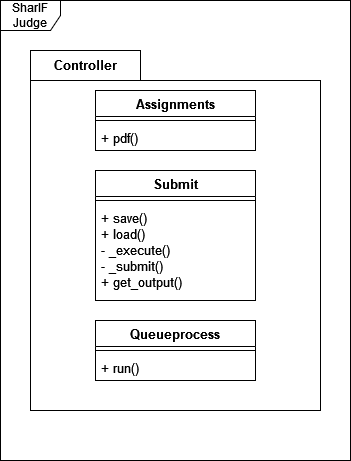
\includegraphics[scale=0.5]{Diagram/Class Diagram Usulan.png}  
	\caption{Diagram kelas perubahan pada SharIF Judge \protect\footnotemark} 
	\label{fig:4:classdiagram} 
\end{figure} 
\footnotetext{Fungsi yang sudah ada tidak ditampilkan, karena sudah terdapat pada gambar \ref{fig:3:classdiagram}}.

Untuk mengimplementasikan fitur-fitur, diperlukan perubahan kode berikut ini pada SharIF Judge. Diagram kelas pada gambar \ref{fig:4:classdiagram} menunjukkan kelas-kelas yang mengalami perubahan 

\subsection{Menampilkan soal}
\label{subsec:4:soal}

SharIF Judge sudah memiliki fitur untuk menyimpan soal dalam bentuk PDF. Untuk melihat soal tersebut, soal harus diunduh terlebih dahulu. Agar pengguna dapat melihat soal secara langsung di halaman Submit, digunakan \textit{library} PDF.js untuk menampilkan PDF soal di halaman Submit.

Untuk menampilkan soal PDF, dilakukan perubahan sebagai berikut:
\begin{itemize}
	\item \textit{Controller} \verb|Assignments|:
    \begin{itemize}
		\item Fungsi \verb|pdf()|: \\ Penambahan kondisi untuk mencegah dialog unduh PDF soal, karena soal akan ditampilkan.
    \end{itemize}
    \item \textit{View} \verb|submit|:
    \begin{itemize}
        \item Penambahan elemen \verb|iframe| sebagai tempat untuk menampilkan PDF soal.
    \end{itemize}
\end{itemize}

\subsection{Mengedit Kode}
\label{subsec:4:editor}

Digunakan \textit{library} Ace untuk menambahkan editor kode pada halaman Submit.

Untuk mengimplementasikan editor kode, perlu dilakukan perubahan sebagai berikut:
\begin{itemize}
    \item \textit{View} \verb|submit|:
    \begin{itemize}
        \item Penambahan elemen \verb|div| sebagai tempat untuk menampilkan editor Ace.
        \item Penambahan \textit{script} untuk konfigurasi Ace.
        \item Penambahan \textit{script} untuk menyesuaikan mode \textit{syntax highlighting} Ace dengan pilihan bahasa pemrograman pada \textit{dropdown}.
    \end{itemize}
\end{itemize}

\subsection{Menyimpan Kode}
\label{subsec:4:simpan}

Seluruh \textit{submission} yang diunggah oleh pengguna pada SharIF Judge akan disimpan pada folder \verb|assignments| sesuai dengan \textit{assignment} dan \textit{problem} yang dipilih. Kode pada editor kode juga akan disimpan pada folder yang sama saat pengguna menekan tombol Save. Kode disimpan sebagai sebuah \textit{file} teks dengan ekstensi txt untuk memudahkan pemuatan kode dan mencegah tersimpannya banyak file dengan ekstensi berbeda.

Untuk menyimpan kode, perlu dilakukan perubahan sebagai berikut:
\begin{itemize}
	\item \textit{Controller} \verb|Submit|:
    \begin{itemize}
		\item Fungsi \verb|save()|: \\ Fungsi baru untuk menyimpan kode pada \textit{file} teks.
    \end{itemize}
    \item \textit{View} \verb|submit|:
    \begin{itemize}
        \item Penambahan elemen \verb|button| untuk menyimpan kode.
        \item Penambahan \textit{script} untuk memanggil fungsi \verb|save()| pada \textit{controller} \verb|Submit| melalui AJAX. 
    \end{itemize}
\end{itemize}

\subsection{Memuat Kode}
\label{subsec:4:muat}

Kode yang sudah tersimpan sebagai akan otomatis dimuat pada editor kode saat pengguna memilih \textit{problem} pada \textit{dropdown}.

Untuk memuat kode, perlu dilakukan perubahan sebagai berikut:
\begin{itemize}
	\item \textit{Controller} \verb|Submit|:
    \begin{itemize}
		\item Fungsi \verb|load()|: \\ Fungsi baru untuk memuat kode dari \textit{file} teks.
    \end{itemize}
    \item \textit{View} \verb|submit|:
    \begin{itemize}
        \item Penambahan \textit{script} untuk memanggil fungsi \verb|load()| pada \textit{controller} \verb|Submit| melalui AJAX. 
    \end{itemize}
\end{itemize}

\subsection{Menjalankan Kode dengan Tes Kasus}
\label{subsec:4:jalan}

Fitur ini memanfaatkan sistem antrean eksekusi kode yang sudah tersedia pada SharIF Judge.
Diperlukan beberapa perubahan agar kode pada editor dapat dimasukkan ke dalam antrean, dijalankan \textit{input} tes kasus, dan \textit{output} dari kode dapat ditampilkan.

Untuk menjalankan kode dengan tes kasus, dilakukan perubahan sebagai berikut:
\begin{itemize}
	\item \verb|tester.sh|:
    \begin{itemize}
        \item Penambahan variabel \verb|EXEC_ONLY| sebagai kondisi untuk menjalankan kode tanpa penilaian.
        \item Penambahan fungsi \verb|shj_log_exec| untuk mencatat hasil \textit{output} dan pesan \textit{error}.
    \end{itemize}
	\item \textit{Controller} \verb|Submit|:
    \begin{itemize}
        \item Fungsi \verb|_execute()|: \\ Fungsi baru untuk memasukkan kode dari editor ke antrean. Fungsi ini dipanggil oleh fungsi \verb|save("execute")|.
        \item Fungsi \verb|get_output()|: \\ Fungsi baru untuk memuat hasil eksekusi kode dari \textit{file} teks.
    \end{itemize}
	\item \textit{Controller} \verb|Queueprocess|:
    \begin{itemize}
        \item Fungsi \verb|run()|: \\ Penambahan kondisi untuk menjalankan \verb|tester.sh| tanpa penilaian.
    \end{itemize}
    \item \textit{View} \verb|submit|:
    \begin{itemize}
		\item Penambahan elemen \verb|textarea| untuk \textit{input}.
		\item Penambahan elemen \verb|textarea| untuk \textit{output}.
        \item Penambahan elemen \verb|button| untuk menjalankan kode.
        \item Penambahan \textit{script} untuk memanggil fungsi \verb|save("execute")| pada \textit{controller} \verb|Submit|.
        \item Penambahan \textit{script} untuk memanggil fungsi \verb|get_output| pada \textit{controller} \verb|Submit|.
    \end{itemize}
\end{itemize}

\subsection{Mengumpulkan Kode Melalui IDE}
\label{subsec:4:kumpul}

Fitur ini memanfaatkan fitur \textit{submit} yang sudah tersedia pada SharIF Judge, namun kode yang digunakan adalah kode yang sudah tersimpan pada editor, sebagai ganti dari unggah \textit{file}. 

Untuk mengumpulkan kode dari editor, perlu dilakukan perubahan sebagai berikut:
\begin{itemize}
	\item \textit{Controller} \verb|Submit|:
    \begin{itemize}
		\item Fungsi \verb|_submit()|: \\ Fungsi baru untuk mengumpulkan kode. Fungsi ini dipanggil oleh fungsi \verb|save("submit")|.
    \end{itemize}
    \item \textit{View} \verb|submit|:
    \begin{itemize}
        \item Penambahan elemen \verb|button| untuk mengumpulkan kode.
        \item Penambahan \textit{script} untuk memanggil fungsi \verb|save("submit")| pada \textit{controller} \verb|Submit|. 
    \end{itemize}
\end{itemize}
